%stpapb

\documentclass[../../main/main.tex]{subfiles}


\begin{document}
\title{STPA on Patrol Base Operations}

%%%%%%%%%%%%%%%% STPA on Patrol Base Operations %%%%%%%%%%%%%%%%
\chapter{STPA/STPA-Sec on Patrol Base Operations}\label{chp:stpapb}
This chapter applies the \gls{stpa}/\gls{stpasec} analysis to the patrol base operations.  The patrol base operations are analyzed at a high level of abstraction and only the actions of the Platoon Leader (PL) and the platoon as a whole are considered.  The limited scope of the analysis serves to demonstrate the \gls{stpa} component of \gls{storm} on the system of interest.  A complete analysis is beyond the scope of this master thesis. 

This chapter describes each of the four steps of the \gls{stpa}/\gls{stpasec} analysis.  The results are discussed in the text and presented in tables.   For a review on the four steps read section \ref{ssec:stpa} of the previous chapter.

%%%%%%%%%%%%%%%% Step 1 %%%%%%%%%%%%%%%%
\section{Step 1: Define The Purpose of The Analysis}\label{chp:stpapb:purpose}
This section describes the first step in the \gls{stpa}/\gls{stpasec} analysis.  It begins with a definition of the stakeholders.  It follows with a description of the goals of the most immediate organizations.  It describes the functional mission analysis for the patrol base operations.  It then describes assumptions about the system and relevant entities.  Next, it describes accidents/losses for the system.  Finally, it describes the system-level hazards/vulnerabilities and constraints.

\paragraph*{Stakeholders}
At the highest level, the stakeholders are the U.S. Government and the Citizens of the United States.  Below that is the U.S. Army and the U.S. Army Rangers.  Depending on the mission, other nations and their citizens may also hold a stake in the activities.  The enemy is also a stakeholder with an adversarial agenda. 

\subsection{Organization FMA}
The two most immediate organization for the parol bae operations are the U.S. Army Rangers and the U.S. Army.  Their goals are stated in table \ref{orgo}
   %%%%%% table: organization goals %%%%%%%%%%
\begin{table}[h!]
\parskip=8pt
\begin{tabular}{||  m {7.5cm}  |  m {7.5cm}  ||}
\hline
\multicolumn{2} {|| c ||} {Organization Goals} \\
 \hline
U.S. Army Rangers	& U.S. Army\\
\hline
"The U.S. Army's mission is to fight and win our Nation?s wars by providing prompt, sustained land dominance across the full range of military operations and spectrum of conflict in support of combatant commanders."
&	
"The Rangers' primary mission is to engage the enemy in close combat and direct-fire battles. This mission includes direct action operations, raids, personnel and special equipment recovery, in addition to conventional or special light-infantry operations."\\
\hline
\end{tabular}
\caption{Organization goals.}
\label{orgo}
\end{table}
   %%%%%% table: organization goals %%%%%%%%%%
%%
\clearpage

\subsection{Patrol Base Operations FMA}
The functional mission analysis for the patrol base operations is shown in table \ref{pbfma}.  This describes what the patrol base operations are, how they are conducted (broadly), and why they are conducted.

   %%%%%% table: PB FMAs  %%%%%%%%%%
\begin{table}[h!]
\parskip=8pt
\begin{tabular}{||  m {3cm}  |  m {12cm}  ||}
\hline
\multicolumn{2} {|| c ||} {Patrol Base Operations FMA} \\
 \hline
What &	establish a security perimeter when a squad or platoon halts for an extended period of time\\
\hline
How	&      planning, reconnaissance, security, control, and common sense\\
\hline
Why	&      avoid detection:
\begin{itemize}
\item hide a unit during a long, 
\item detailed reconnaissance; 
\item perform maintenance on weapons, 
\item equipment, eat, and rest; 
\item plan and issue orders; 
\item reorganize after infiltrating an enemy area; 
\item establish a common base from which to execute several consecutive or concurrent operations.
\end{itemize}\\
\hline
\end{tabular}
\caption{Patrol Base Operations Functional Mission Analysis.}
\label{pbfma}
\end{table}
   %%%%%% table: PB FMAs  %%%%%%%%%%
%%
\clearpage
\subsection{Assumptions about The System}
This analyzes relies on the following assumptions about the model of patrol base operations.

\begin{itemize}
\item Mission is decided by higher-ups and is provided as an input to the patrol base operations.
\item Mission is not changeable by the patrol base itself (exceptions are mission-specific).
\item Soldiers are deemed fit for duty before the mission commences.   (There may be exceptions.)
\item Soldiers are battle ready, but may not be fully mission capable (i.e., soldiers may require additional equipment and preparation that is mission-specific and determined after the mission is received).
\item The patrol base operations begin when the platoon (or patrol) leader receives order that there will be a mission.
\item The patrol base operations end when the patrol returns to the larger unit and has completed any debriefing required by the mission.
\item Other inputs to the system are intelligence from the larger unit (higher-up HQ), intelligence from other units (if applicable), and intelligence gathered during the mission from the mission itself. 
\item Feedback is received from the platoon regarding carrying out orders and from the operations themselves regarding completion of tasks, etc.  
\item Adversary also may input information to the platoon leader (by interfering with communications from higher-up HQ), to the platoon soldiers (by interfering with intra-patrol communications), and to the operations themselves (by disrupting on the operations in various forms, including contact).
\end{itemize}


\subsection{System Entities}
The following entities are defined in the U.S. Ranger Handbook for the patrol base operations.  
\begin{itemize}
\item HQ: PL, PSG, Medic, FO, RTO, HWSQ
\item Squad Leaders
\item Fire Team Leaders
\item Buddy Team
\item Soldiers
\item Adversary (enemy)
\end{itemize}

The platoon leader (Platoon Leader --PL) is the only entity specifically referred to in this limited-scope analysis.  The platoon sergeant (PSG) is the assistant to the platoon leader.  The patrol base head quarters (HQ) consists of the PL, PSG, Medic, forward observer (FO), radio telephone operator (RTO), and the heavy weapons squad leader (HWSQL).  Below the HQ are four squad leaders.\footnote{This is only true for platoon sized patrol base operations.  Squad-sized patrol base operations consist of only one squad.}  Each squad is comprised of two fire teams.  Each fire time is compose of two or more buddy teams.  Each buddy team is composed of two soldiers (buddies).

%%
\clearpage
\subsection{Accidents/Losses}
Accidents/losses for the patrol base operations are shown in table \ref{losses}.
   %%%%%% table: Accidents/Losses  %%%%%%%%%%
\begin{table}[h!]
\parskip=8pt
\begin{tabular}{||  m {2cm}  |  m {13cm}  ||}
\hline
\multicolumn{2} {|| c ||} {Accidents/Losses} \\
\hline
	&Description\\
\hline
L1	&MIA, KIA, WIA, CIA\footnote{MIA = missing in action; KIA = killed in action; WIA = wounded in action; CIA = captured in action.}\\
\hline
L2	&Wrong mission\\
\hline
L3	&Mission Failure\\
\hline
L4	&Negative publicity/exposure/unwanted attention\\
\hline
L5	&Equipment loss/damage/capture by enemy\\
\hline
L6	&Civilian casualties/disruption to local population\\
\hline
L7	&Insufficient communications with high-up HQ\\
\hline
\end{tabular}
\caption{System accidents/losses.}
\label{losses}
\end{table}
   %%%%%% table: Accidents/Losses  %%%%%%%%%%

%%
\clearpage
\subsection{System-level Hazards/Vulnerabilities And Constraints}
The system-level hazards/vulnerabilities are described in the second column in table \ref{hazards}.  The associated accidents/losses for each hazard are shown in the next column.  These are linked to system-level constraints in the last column.   

  %%%%%% table: System-level hazards  %%%%%%%%%%
\begin{table}[h!]
\parskip=8pt
\begin{tabular}{|  m {0.7cm}  |  m {4.5cm} |  m{3.5cm}   |   m {0.7cm} |  m {4.5cm}   |}
\hline
\multicolumn{5}{| c |}{Hazards/Vulnerabilities and constraints}\\
\hline
\multicolumn{2}{| c |}{System-level Hazards/Vulnerabilities} & \multicolumn{1}{| c |}{Accidents/Losses} & \multicolumn{2}{| c |}{System-level Constraints}\\
\hline
H1    &Insufficient planning		&L1, L2, L3, L4, L5, L6, L7	&SC1	&Plan sufficiently\\
\hline
H2	&Insufficient reconnaissance/intelligence	&L1, L2, L3, L4, L5, L6, L7	&SC2	&Reconnoiter sufficiently\\
\hline
H3	&Insufficient security			&L1 ,L3, L4, L5, L6		&SC3	&Provide sufficient security\\
\hline
H4	&Insufficient control			&L1, L2, L3, L4, L5, L6 ,L7	&SC4	&Maintain adequate control\\
\hline
H5	&Insufficient common sense	&L1, L2, L3, L4, L5, L6, L7	&SC5	&Use common sense\\
\hline
H6	&Insufficient leadership		&L1, L2, L3, L4, L5, L6, L7	&SC6	&Establish sufficient leadership\\
\hline
H7	&Insufficient communication with higher-HQ	&L1, L2, L3, L4, L5, L6, L7	&SC7	&Maintain sufficient communications with higher-HQ\\
\hline
H8	&Insufficient haste			&L1, L3	&SC8	&Maintain appropriate pace\\
\hline
H9	&Disregard for Rules of Engagement  &L4, L6	&SC9	&Follow Rules of Engagement\\ 
\hline
\end{tabular}
\caption{System-level hazards/vulnerabilities and constraints.}
\label{hazards}
\end{table}
  %%%%%% table: System-level hazards  %%%%%%%%%%
  
A more in-depth analysis would return to this table and generate refined hazards/vulnerabilities and constraints.  For example, H1 could be refined to H1.1 insufficient reconnaissance, H1.2 mission objectives not clear, H1.3 insufficient time for completing plan, etc..  For the constraints, SC1.1 reconnoiter efficiently, SC1.2 confirm mission objectives, SC1.3 use time efficiently, etc..
  
%%
\clearpage
%%%%%%%%%%%%%%%% Step 2 %%%%%%%%%%%%%%%
\section{Step 2: Model The Control Structure}\label{chp:stpapb:control}
This section first breaks the patrol base operations down into phases.  It hen describes the system controllers and their process models.  It then describes the control actions for each controller.  Finally, it presents a diagram of the functional control model.

\subsection{Phases of The Patrol Base Operations}
Figure \ref{pbtoplevel2stpa} shows the patrol base operations broken down into six phases.   This is a simplified first approximation of the patrol base operations and is very abstract.  For the purposes of this analysis, transitions among phases of the operations are indicated by the Platoon Leader who is responsible for the success of the mission as a whole.  

\begin{table}[ht!]
\begin{center}
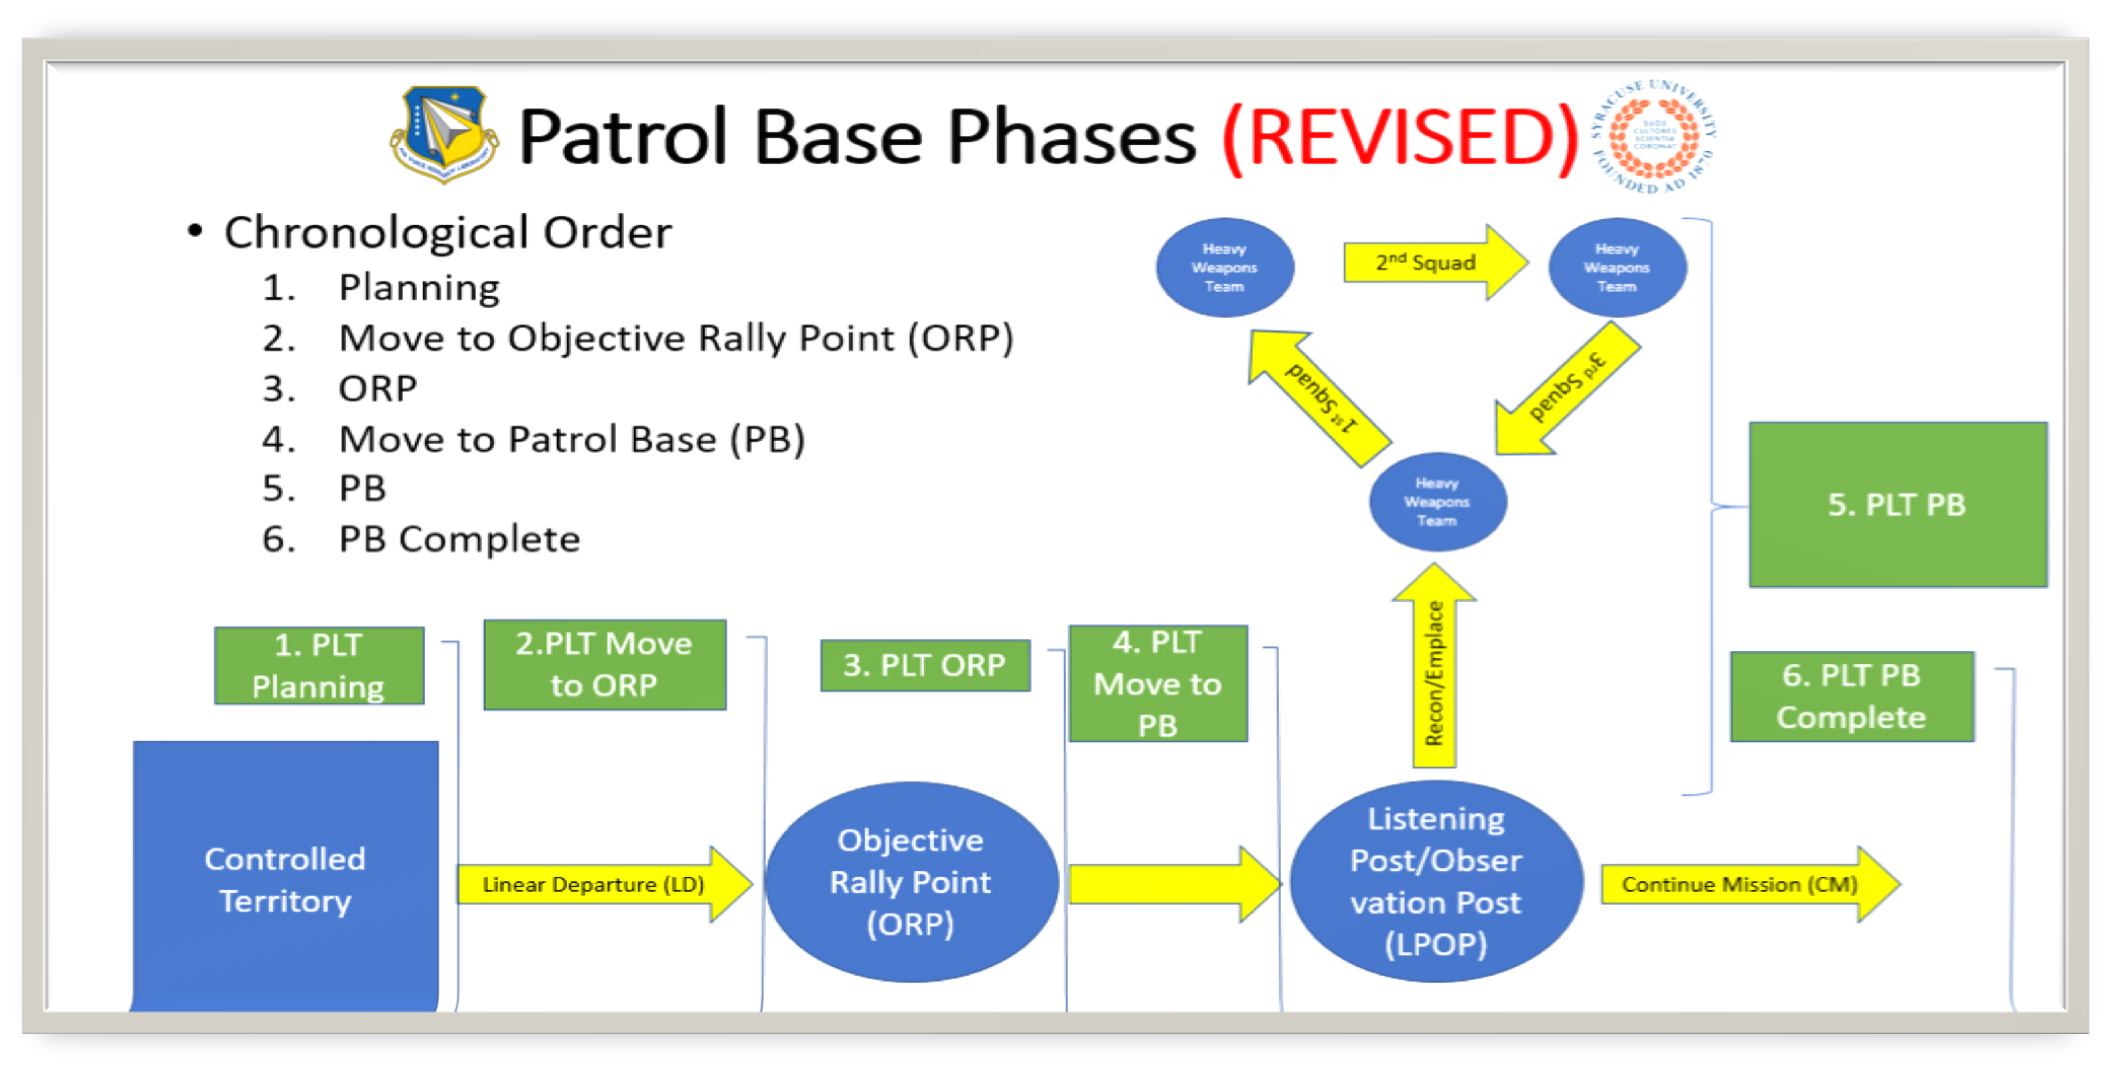
\includegraphics[width=\linewidth]{../figures/pbtoplevel}
\caption{Scenarios for UCA E1A3.}
\label{pbtoplevel2stpa}
\end{center}
\end{table}
%%
\clearpage

\subsection{Controllers And Process Models}
The controllers and their process models are shown in table \ref{controlprocess}.  
 %%%%%% table: Controllers Processes %%%%%%%%%%
\begin{table}[h!]
\parskip=8pt
\begin{tabular}{|  m {3cm}  |  m {3cm}  |  m {3cm}     |  m {5cm}   |}
\hline
\multicolumn{4}{| c |}{Controllers And Process Model}\\
\hline
Controller & Model & Variables & Values\\
\hline
\multirow{2}{3cm}{Platoon Leader}	& Patrol Base \newline Status	& State	 &
\begin{itemize}
\item PLAN_PB
\item MOVE_TO_ORP
\item CONDUCT_ORP
\item MOVE_TO_PB
\item CONDUCT_PB
\item COMPLETE_PB
\item ABORT_PB
\end{itemize}\\
\cline{2-4}
      & Policy  & Authorized &
 \begin{itemize}
\item True
\item False
\end{itemize}\\
\hline
Platoon	& Authentication Model	& Authenticated	 &
\begin{itemize}
\item True
\item False
\end{itemize}\\
\hline
Adversary	& Threat Model	& To be \newline determined & to be determined\\
\hline
\end{tabular}
\caption{Controllers and process model.}
\label{controlprocess}
\end{table}
 %%%%%% table: Controllers Processes %%%%%%%%%%
 
 Each controller has a one or more models of the patrol base operations that governs her decisions and actions.  Each model has a variable that can take on one of several values.  For example, the Platoon Leader has a model of the Patrol Base Status.  The status is the State of the system.  For example, the State could be PLAN_PB or MOVE_TO_ORP.   
 
 There are three controllers: the Platoon Leader, the platoon, and the adversary (enemy).  The Platoon Leader is the top controller. She issues orders to the subordinates (the platoon) based on her knowledge of the status and policy of the operations.  The platoon authenticates the Platoon Leader and either executes the orders or discards the commands.
 %%
\clearpage

\subsection{Control Actions}
Each controller has its own set of actions (commands, etc.) that it can issues.  The control actions for each principal are listed below.  
\begin{itemize}
\item Platoon Leader
\begin{itemize}
\item PL says planComplete (same as crossLD)
\item PL says conductORP
\item PL says moveToPB
\item PL says completePB
\item PL says reactToContact
\item PL says returnToBase
\item PL says changeMission
\end{itemize}
\item Platoon
\begin{itemize}
\item exec(crossLD) (same as planComplete)
\item exec(conductORP)
\item exec(moveToPB)
\item exec(completePB)
\item exec(reactToContact)
\item exec(returnToBase)
\item exec(changeMission)
\end{itemize}

\end{itemize}

For example, the Platoon Leader may determine (based on policy, etcl), that the planning phase is complete.  She may then indicate this with the statement \textit{PL says planComplete}.\footnote{crossLD = cross line of discrimination.  Depending on the model, this would occur after planning.  It would transition the patrol into the MOVE_TO_ORP phase of the operations.  A description of this works is reserved for chapter \ref{}chp:pb.}

\subsection{Functional Control Structure}
%%
\clearpage

\begin{figure}[ht!]
\begin{center}
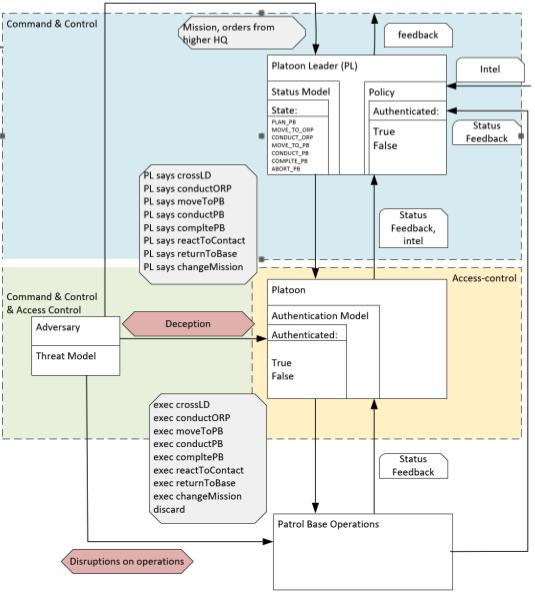
\includegraphics[width=0.7\linewidth]{../figures/controlstr1}
\caption{Control structure for patrol base operations.}
\label{controlstr1}
\end{center}
\end{figure}

%%
\clearpage

%%%%%%%%%%%%%%%% Step 3 %%%%%%%%%%%%%%%%
\section{Step 3: Identify Unsafe Control Actions (UCAs)}\label{chp:stpapb:uca}
The Thomas methods is used to identify \glspl{uca}.

\subsection{Unsafe Control Actions (UCAs): Thomas Model}
%%
\clearpage
\paragraph*{PL says planComplete}
The Thomas method for delineating \glspl{uca} for \textit{PL says planComplete} are shown in figure \ref{UCAPLsays}.
\begin{table}[ht!]
\begin{center}
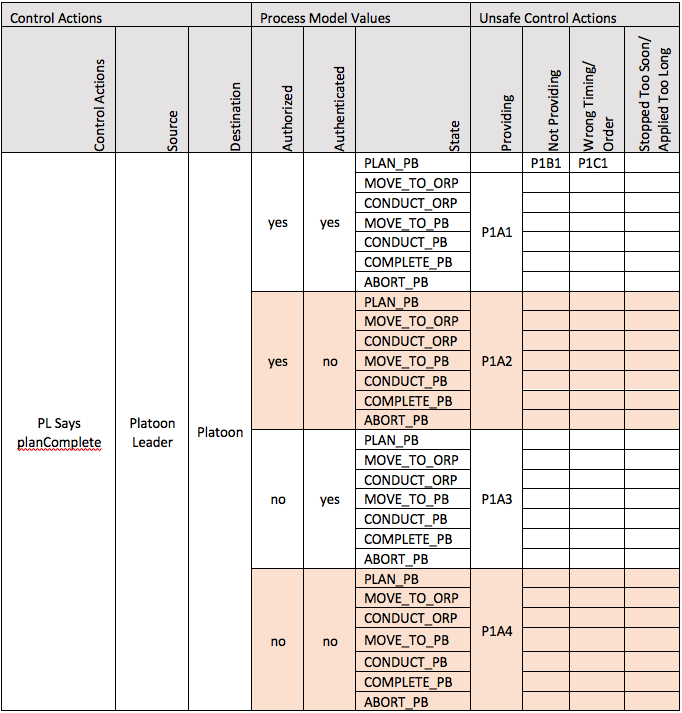
\includegraphics[width=\linewidth]{../figures/UCAPLsays}
\caption{Unsafe control actions \glspl{uca} for control action "PL says planComplete."}
\label{UCAPLsays}
\end{center}
\end{table}

%%
\clearpage
\paragraph*{exec(planComplete)}
The Thomas method for delineating \glspl{uca} for \textit{exec(planComplete)} are shown in figure \ref{UCAPLsays}.
\begin{table}[ht!]
\begin{center}
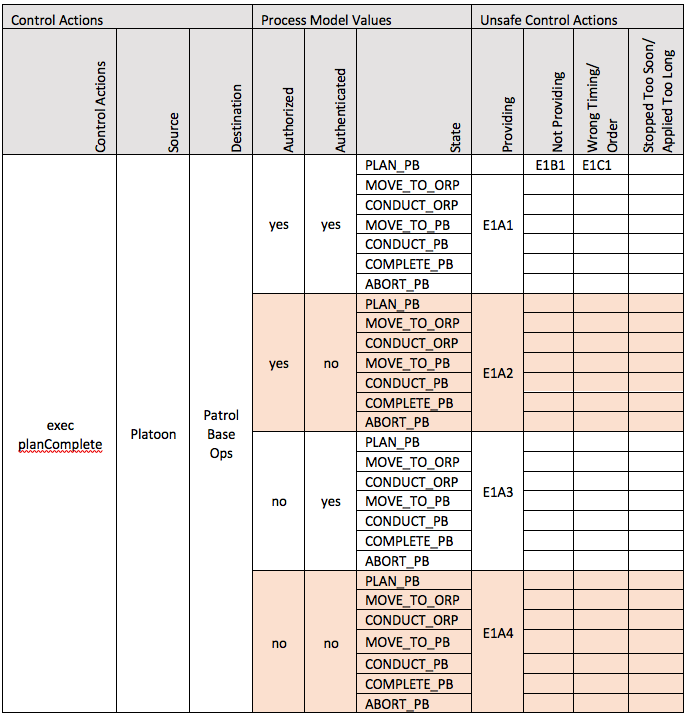
\includegraphics[width=\linewidth]{../figures/UCAexecplan}
\caption{Unsafe control actions \glspl{uca} for control action "exec(planComplete)."}
\label{UCAexecplan}
\end{center}
\end{table}

%%
\clearpage
\paragraph*{discard(anyCommand)}
The Thomas method for delineating \glspl{uca} for \textit{discard{anyCommand}} are shown in figure \ref{UCAPLsays}.
\begin{table}[ht!]
\begin{center}
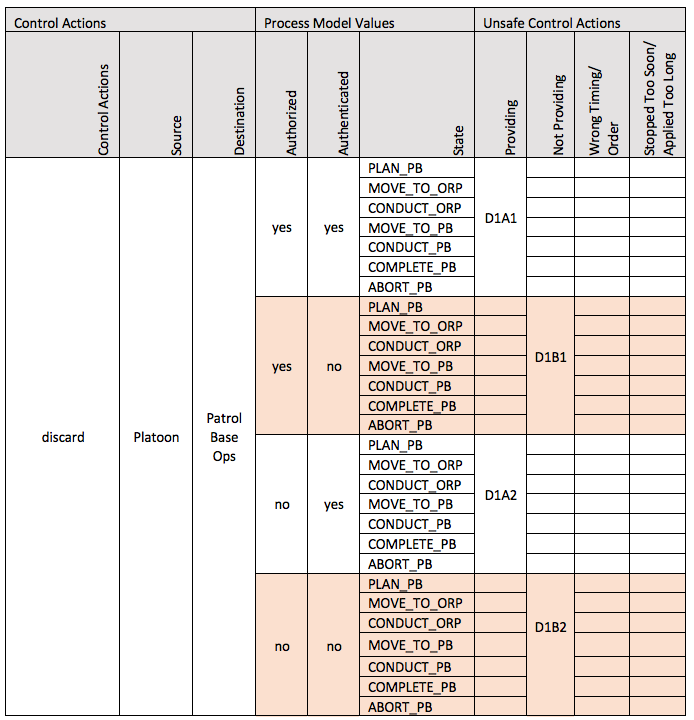
\includegraphics[width=\linewidth]{../figures/ucadiscards}
\caption{Unsafe control actions \glspl{uca} for control action "discard(anyCommand)."}
\label{UCAdiscard}
\end{center}
\end{table}
%%
\clearpage
%%%%%%%%%%%%%%%% Step 4 %%%%%%%%%%%%%%%%
\section{Step 4: Identify Loss Scenarios}\label{chp:stpapb:scenarios}
\subsection{Scenarios}

\subsubsection*{Pl says planComplete}
%%
\clearpage
\paragraph*{P1B1/P1C1: state = PLAN_PB, Authorized = Yes, Authenticated = Yes}

\begin{table}[ht!]
\begin{center}
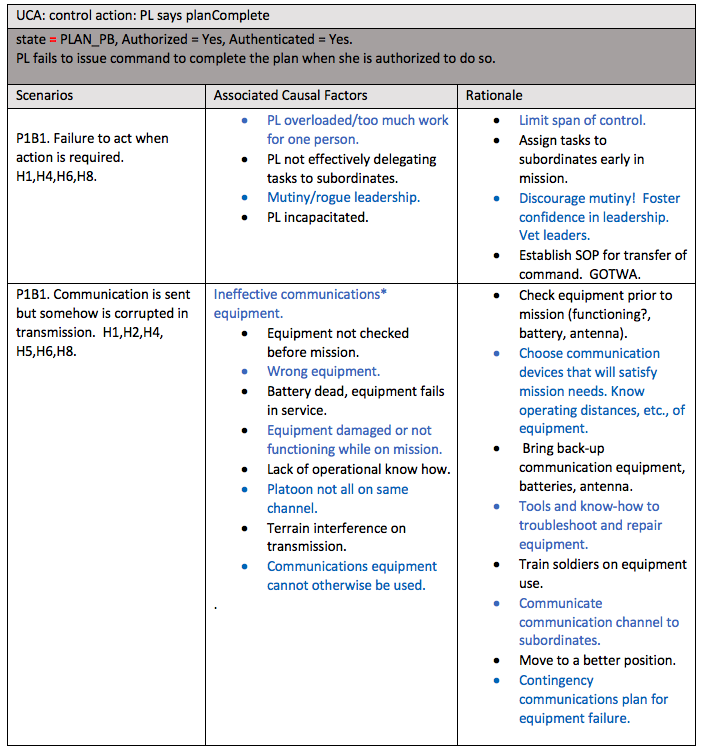
\includegraphics[width=\linewidth]{../figures/ucap1b1}
\caption{Scenarios for UCA P1B1.}
\label{ucap1b1}
\end{center}
\end{table}
%%
\clearpage


\begin{table}[ht!]
\begin{center}
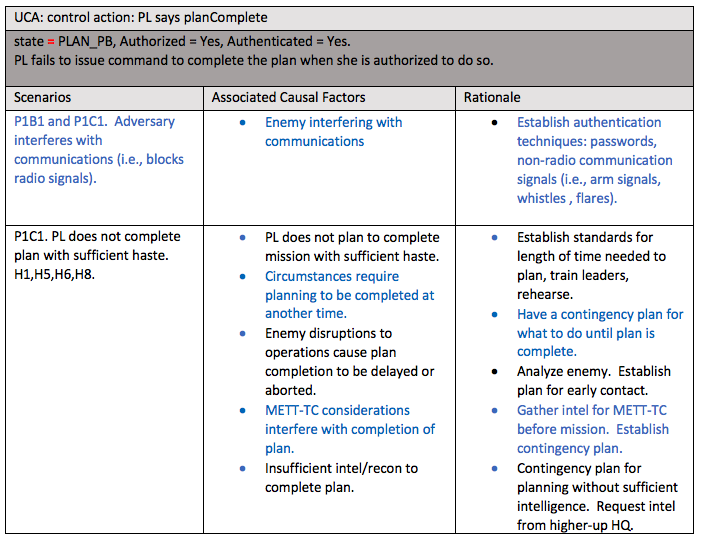
\includegraphics[width=\linewidth]{../figures/ucap1b1p1c1}
\caption{Scenarios for UCA P1B1/P1C1.}
\label{ucap1b1p1c1}
\end{center}
\end{table}
%%
\clearpage



\paragraph*{P1A1: state  = PLAN_PB, Authorized = Yes, Authenticated = Yes}


\begin{table}[ht!]
\begin{center}
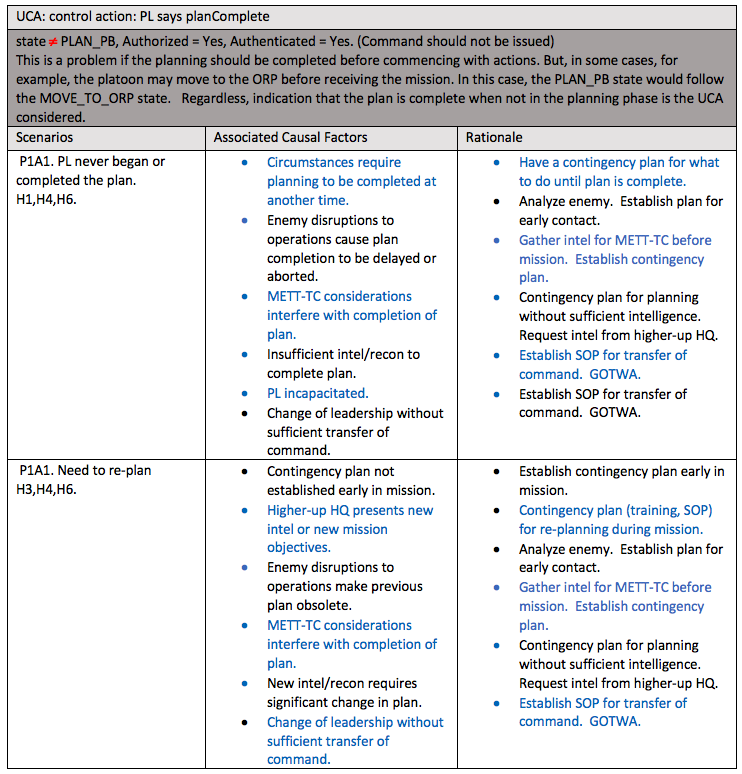
\includegraphics[width=\linewidth]{../figures/ucap1a1}
\caption{Scenarios for UCA P1A1.}
\label{ucap1a1}
\end{center}
\end{table}
%%
\clearpage
\paragraph*{P1A2: state  = any state, Authorized = Yes, Authenticated = No}

\begin{table}[ht!]
\begin{center}
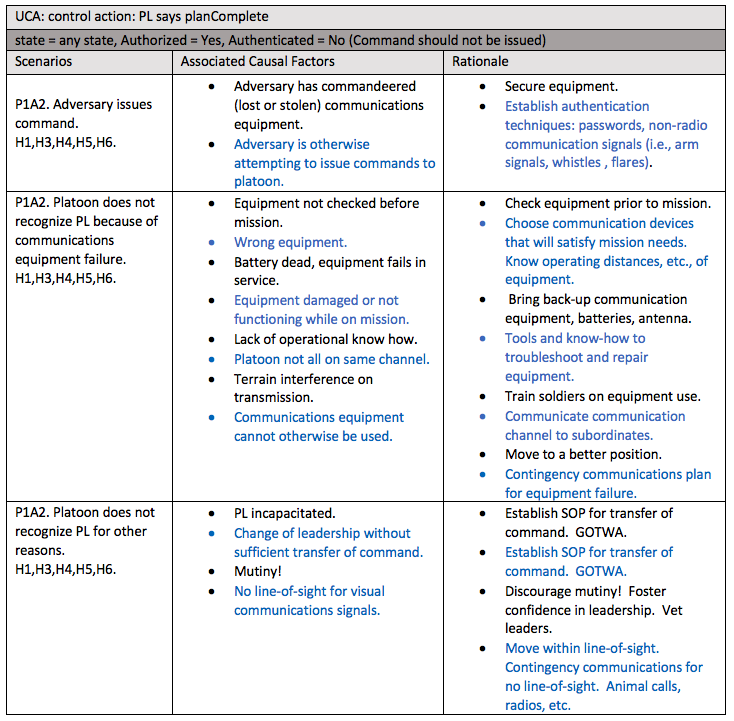
\includegraphics[width=\linewidth]{../figures/ucap1a2}
\caption{Scenarios for UCA P1A2.}
\label{ucap1a2}
\end{center}
\end{table}

%%
\clearpage
\paragraph*{P1A3: state  = any state, Authorized = No, Authenticated = Yes}

\begin{table}[ht!]
\begin{center}
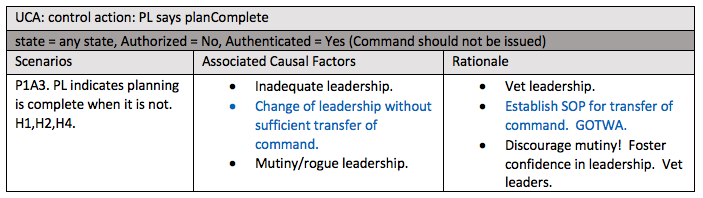
\includegraphics[width=\linewidth]{../figures/ucap1a3}
\caption{Scenarios for UCA P1A3.}
\label{ucap1a3}
\end{center}
\end{table}

%%
\clearpage


\paragraph*{P1A4: state  = any state, Authorized = No, Authenticated = No}

\begin{table}[ht!]
\begin{center}
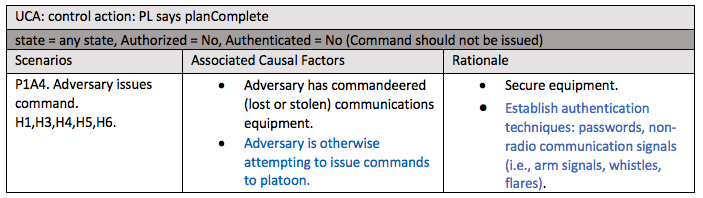
\includegraphics[width=\linewidth]{../figures/ucap1a4}
\caption{Scenarios for UCA P1A4.}
\label{ucap1a4}
\end{center}
\end{table}
%%
\clearpage


\subsubsection*{exec(planComplete)}
\paragraph*{E1B1/E1C1: state = PLAN_PB, Authorized = Yes, Authenticated = Yes}

\begin{table}[ht!]
\begin{center}
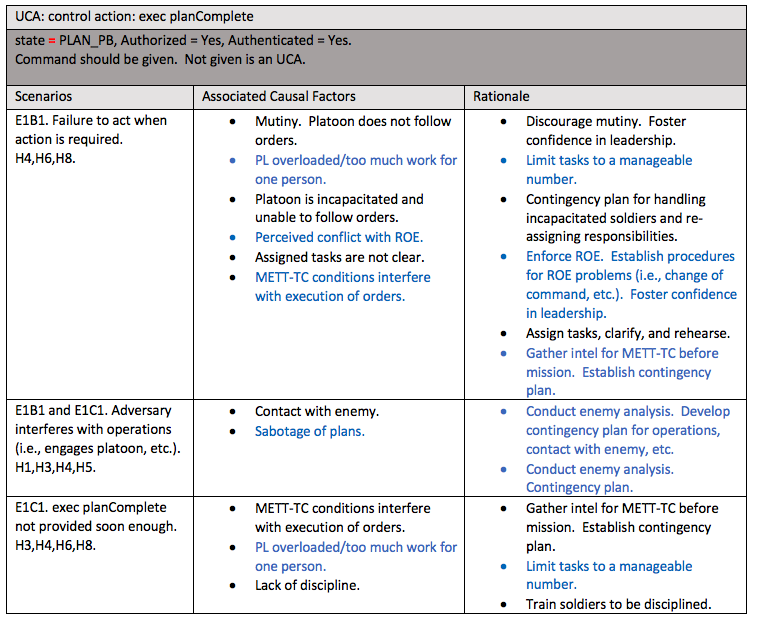
\includegraphics[width=\linewidth]{../figures/ucae1b1e1c1}
\caption{Scenarios for UCAs E1B1 and E1C1.}
\label{ucae1b1e1c1}
\end{center}
\end{table}
%%
\clearpage

\paragraph*{E1A1: state  $\neq$ PLAN_PB, Authorized = Yes, Authenticated = Yes}

\begin{table}[ht!]
\begin{center}
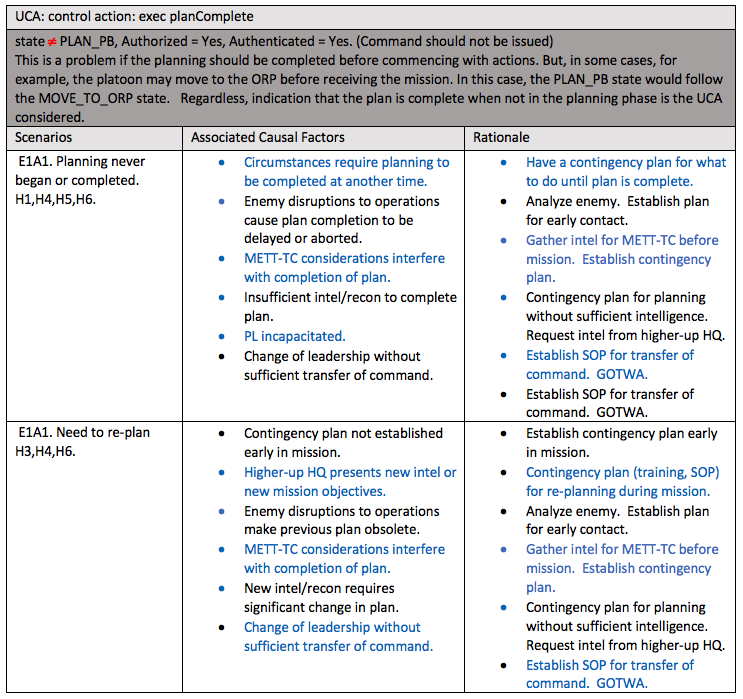
\includegraphics[width=\linewidth]{../figures/ucaea1}
\caption{Scenarios for UCA E1A1.}
\label{ucaea1}
\end{center}
\end{table}
%%
\clearpage
\paragraph*{E1A2: state  = any state, Authorized = Yes, Authenticated = No}
\begin{table}[ht!]
\begin{center}
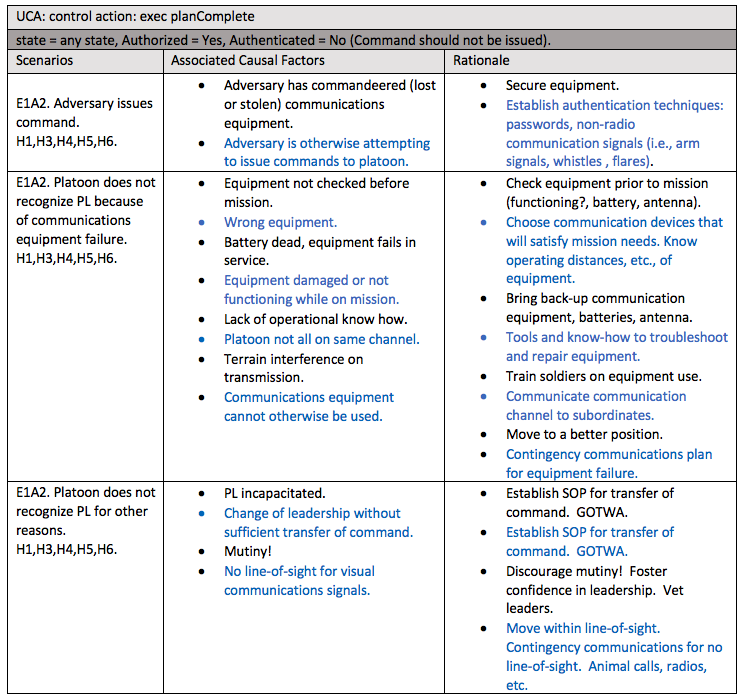
\includegraphics[width=\linewidth]{../figures/ucae1a2}
\caption{Scenarios for UCA E1A2.}
\label{ucae1a2}
\end{center}
\end{table}
%%
\clearpage

\paragraph*{E1A3: state  = any state, Authorized = No, Authenticated = Yes}

\begin{table}[ht!]
\begin{center}
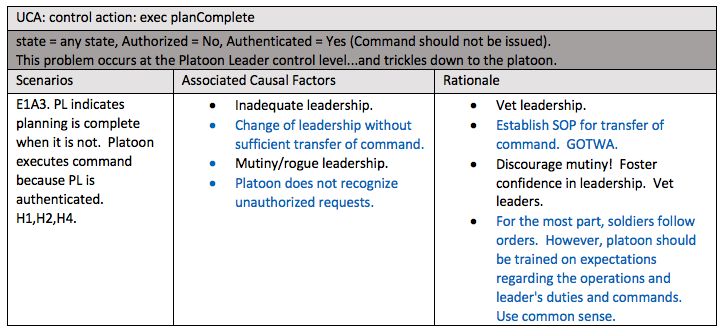
\includegraphics[width=\linewidth]{../figures/ucae1a3}
\caption{Scenarios for UCA E1A3.}
\label{ucae1a3}
\end{center}
\end{table}
%%
\clearpage


\paragraph*{E1A4: state  = any state, Authorized = No, Authenticated = No}

\begin{table}[ht!]
\begin{center}
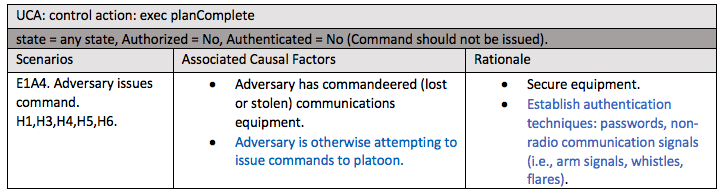
\includegraphics[width=\linewidth]{../figures/ucae1a4}
\caption{Scenarios for UCA E1A3.}
\label{ucae1a4}
\end{center}
\end{table}
%%
\clearpage


\subsubsection*{discard(anyCommand)}

\begin{table}[ht!]
\begin{center}
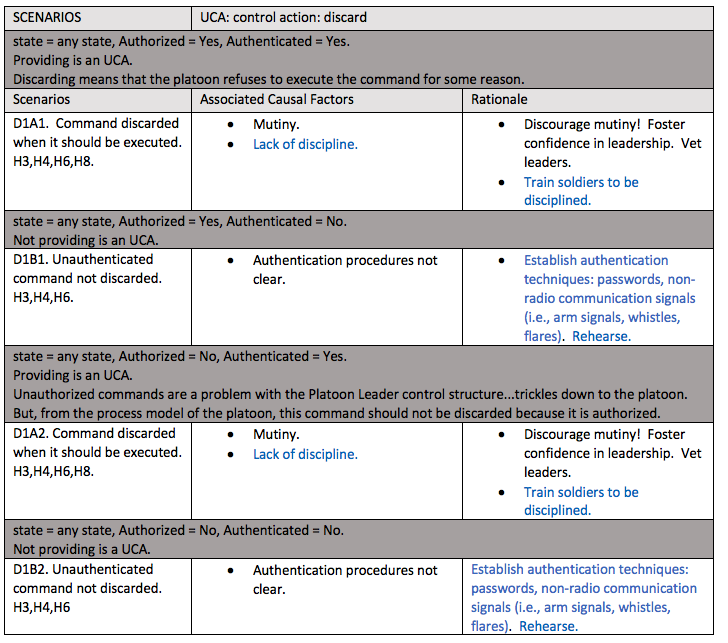
\includegraphics[width=\linewidth]{../figures/ucadiscard}
\caption{Scenarios for UCA for discard on all commands (D1A1 through D1A4).}
\label{ucadiscard}
\end{center}
\end{table}
%%
\clearpage

%%%%%%%%%%%%%%%% Discussion %%%%%%%%%%%%%%%%
\section{Discussion And Conclusions}\label{chp:stpapb:discuss}


\end{document}